\documentclass[11pt,a4paper,twocolumn]{article}

\usepackage{graphicx}
\usepackage{float}
\usepackage{caption}
\usepackage{fancyhdr}
\graphicspath{ {images/} }

\newcommand{\source}[1]{\vspace{-10pt}  \caption*{{\em Source}: {#1}} }

\title {Influencing Game Dynamics In A Roguelike Game Through Procedural Content Generation Using Genetic Algorithm}
\author {Josiah Maius S. Ebia \\ 
23A15 Victoria de Manila, 1655 Taft Ave., Manila \\
09275458093 \\
josiah.maius.ebia@gmail.com \\
\\
John Carl R. Manalansan \\ 
Barangay 20, Zone 2, Porvenir St., Pasay \\
09776892834 \\
manalansanjohncarl@gmail.com \\
\\
John Kenneth V. Bunagan \\ 
B4, L8, Caluya St., Greatwoods Subd., Bahayang Pag-asa, Bacoor, Cavite \\
09952059624 \\
johnkenneth.bunagan0219@gmail.com \\
\\
Kate Danielle D. Guino \\ 
883-J Cristobal St., Paco, Manila \\
09971055834 \\
kdguino@gmail.com  }

\date{October 2017}

\begin{document}


\maketitle

\newpage

\section{Introduction}
\subsection{Background}
Procedural content generation (PCG) has been a very popular technique in game design since the past decades. It lets game designers and developers add more replayabilty to their game. Procedurally generating content will always lead to mostly new and exciting playthroughs everytime the player hits the "new game" button. For developers, this design technique saves much more time, in the long run, and resources when creating a game with large amounts of content e.g. {\em The Elder Scrolls: Arena}\cite{Bethesda}. 

One of the most popular uses of PCG in game development are in {\em roguelike} games. Roguelikes are games with core mechanics similar to the game {\em Rogue}\cite{Toy}, which was released on 1980. Some of the key features of Roguelikes are procedural generation, permadeath, and character progression \cite{Almgren}. Roguelikes, being primarily PCG-based in terms of design, makes it a practical game genre to work on for research titles on PCG and game design theory such as presented in this paper.

Game dynamics are the emergent behavior from the player and game elements when the game's mechanics, which are the particular components of the game such as the game's rules and A.I., are implemented. An example of this is when a player runs from an enemy when her health points are lower than the enemy, or when a player tries to find a key when discovering that a door that is the goal is locked.

In this research, we looked into influencing the emergent behaviors in the game that is game dynamics through procedural generation. This will allow a more personalized play experience for the player, and at the same time, staying true to the unforgiving nature of roguelikes since the game's environment will start to adapt against the player as she progresses. 

To accomplish this, we used genetic algorithms, which is a kind of evolutionary algorithm that is inspired by natural selection, to evolve specified elements in the generated content of the game's level depending on the results of the previous level of the game. Lastly, we designed and developed {\em Fireflies}, an experimental 2D roguelike game, to demonstrate the objectives of this research.

\subsection{Significance of the Study}
This study can be a model for game designers and developers to improve their understanding on the effectiveness of genetic algorithms in designing roguelike games. It shows a specific way, using genetic algorithms, on how to make the procedural content generated in roguelike games and the play experience delivered to the player be personalized and more meaningful.
This study can also be a framework for students and future researchers in conducting research on game design, procedural content generation, and genetic algorithms.

\subsection{Scope and Limitation of the Study}

The focus of this research is to utilize genetic algorithms in the procedural generation of content to influence the game dynamics (emergent behavior) in the {\em Fireflies} game, giving the player a more personalized experience and at the same time staying true to the nature of roguelikes being both very challenging and fun. 
Although the methods used in this research project is promising for very challenging games such as that of the roguelike genre, this paper doesn't promise to be as effective on other less challenging games in providing the amount of fun that this can give when applied on roguelikes.

\section{Review of Related Literature}

\subsection{Procedural Content Generation}

Procedural content generation (PCG) simply refers to the algorithmic generation of game content with limited or no human contribution \cite{Togelius1, Togelius2}. PCG has been used for decades in the games industry. It was primarily used to deliver more content in games that runs in a very limited hardware, popular examples of this are {\em Rogue}\cite{Toy} and {\em The Elder Scrolls: Arena}\cite{Bethesda}. In both games mentioned, the developers used PCG to generate game content that would be too large for the existing technology in their time to store and run in memory if predefined. Today, PCG is mainly used to give games more replay value and varied content.

\subsection{Roguelike Games}

\begin{figure}[H]
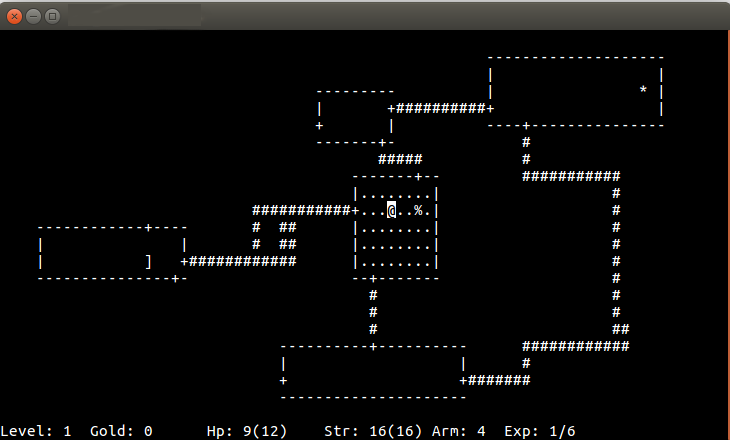
\includegraphics[width=7.5cm]{rogue_screenshot.png}
\centering
\captionsetup{justification=centering}
\caption{A screenshot of the game {\em Rogue} running on the Ubuntu Linux terminal.}
\label{fig:rogue}
\end{figure}

Roguelikes are games whose core features are similar to those of the game {\em Rogue}\cite{Toy}, thus the name. {\em Rogue} was developed by Michael Toy and Glenn Wichman which was initially released on 1980. It was a turn-based dungeon-crawler that used ASCII characters to represent its game content.

{\em The Berlin Interpretation}\cite{Berlin} split the factors that defines roguelikes into two, the {\em high value factors} and {\em low value factors}, the factors listed under the former are the more important features to be found in roguelikes than the those under the latter which are likely optional. The following are the high value factors of roguelikes according to The Berlin Interpretation, in no specific order of importance:
\begin{itemize}
  \item Random environment generation
  \item {\em Permadeath} (which stands for permanent death)
  \item Turn-based
  \item Grid-based
  \item Non-modal
  \item Complexity
  \item Resource Management
  \item {\em Hack'n'Slash}
  \item Exploration and discovery
\end{itemize} 
Below are the low value factors, in no specific order of importance:
\begin{itemize}
  \item Single player character
  \item Monsters are similar to players
  \item Tactical challenge
  \item ASCII display
  \item Dungeons
  \item Numbers
\end{itemize} 


\subsection{Game Dynamics}
According to the MDA ({\em Mechanics-Dynamics-Aesthetics}) framework \cite{Hunicke}, the consumption of games are broken down into three distinct components which are rules, system, and {\em fun}, and their design counterpart are mechanics, dynamics, and aesthetics. According to Hunicke et al.\cite{Hunicke}, mechanics are defined as the particular components of the game, at the level of data representation and algorithms; the dynamics are the run-time behavior of the mechanics acting on player inputs and each others’ outputs over time; and aesthetics are the desirable emotional responses evoked in the player, when she interacts with the game system.

\begin{figure}[H]
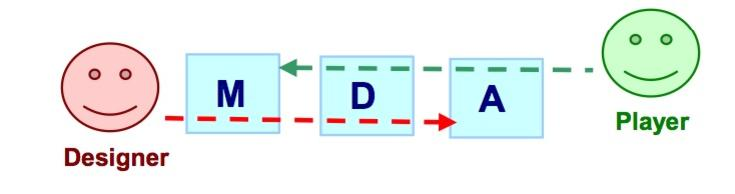
\includegraphics[width=7.5cm]{MDA.jpg}
\centering
\captionsetup{justification=centering}
\caption{The MDA framework. Shows the difference in perspective of the player (consumer) and the designer (or developer).}
\label{fig:mda}
\end{figure}



\subsection{Genetic Algorithms}

Genetic algorithms (GA) are stochastic, parallel search algorithms based on the mechanics of natural selection and evolution \cite{Cole, Whitley}. It was first introduced by John Holland on 1992 \cite{Holland} which is very similar to Darwin's theory of natural selection.

A genetic algorithm starts off with a population of elements, or {\em chromosomes}, which carry their own genetic information commonly referred to as {\em genes}. The algorithm will then evaluate the {\em fitness} of each of the chromosomes in the population, the evaluation function of a genetic algorithm depends on the problem being solved. A chromosome's {\em fitness value} will determine its likelihood of being picked as a {\em parent} for the new generation of likely more optimal chromosomes. When the parent chromosomes are picked the algorithm will perform {\em crossover} and {\em mutation}. The {crossover} function will combine genes from the parent chromosomes to form a new chromosome for the next generation, a {\em mutation} may occur once the crossover is done which will mutate a certain gene that is unique from its parents.

The above explaination may also be described as: 
\[P = \{ x | x \mbox{ is the return value of } f(c_1, c_2, ..., c_n)\}\] 
where \(f\) is a genetic function that takes \(n\) number of chromosome \(c\) and returns a child chromosome \(x\), and \(f\) runs \(N\) times where \(N\) is the required number of chromosomes for the population set \(P\) in the next generation. The genetic algorithm stops when it produces the most optimal result that satisfies the problem. 


\section{Methodology}

\subsection{The {\em Fireflies} game}

{\em Fireflies} is an experimental 2D turn-based roguelike game. In {\em Fireflies}, the player is thrown in a series of procedurally generated dungeon levels with harmful and helpful game elements such as enemies and loot. The main objective of the player is to utilize her resources and strategize to find a way to the goal of each level and finally see end game. 

{\em Fireflies} features procedurally generated levels, this means that certain parameters {\em (e.g. the x and y coordinates of the objects)} of every game object in every new level that the player enters isn't predefined and will not be always the same. Each dungeon level generated will contain matching rooms and corridors, enemies, loot, and a goal.

The game is heavily turn-based, all actors in the game including the player have one action per turn. Every turn, an actor either attacks or moves to a tile to change its position, as shown in Figure \ref{fig:turnflow}. The turn of every other actor in the game starts after the player finishes her turn.

\begin{figure}[h]
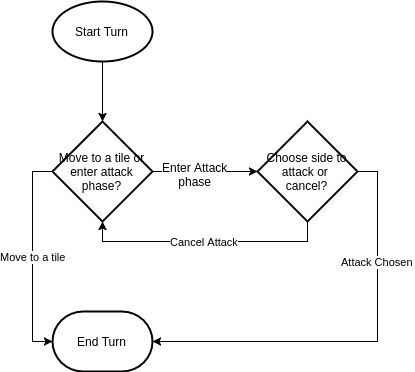
\includegraphics[width=7.5cm]{turn-flow.png}
\centering
\captionsetup{justification=centering}
\caption{The general flow of an actor's turn in the game.}
\label{fig:turnflow}
\end{figure}

During the player's turn, she can choose to attack instead of moving to another tile. This will cause the player to enter the attack phase, where a marker will appear one(1) tile from her position and she may choose to attack one tile north, east, south, or west, this is shown in Figure \ref{fig:combatphase}. The player may also cancel the attack and return to her normal state, doing this will not cost the player a turn and she may either choose to move or attack again.

\begin{figure}[h]
\centering
\hspace*{-.3cm}
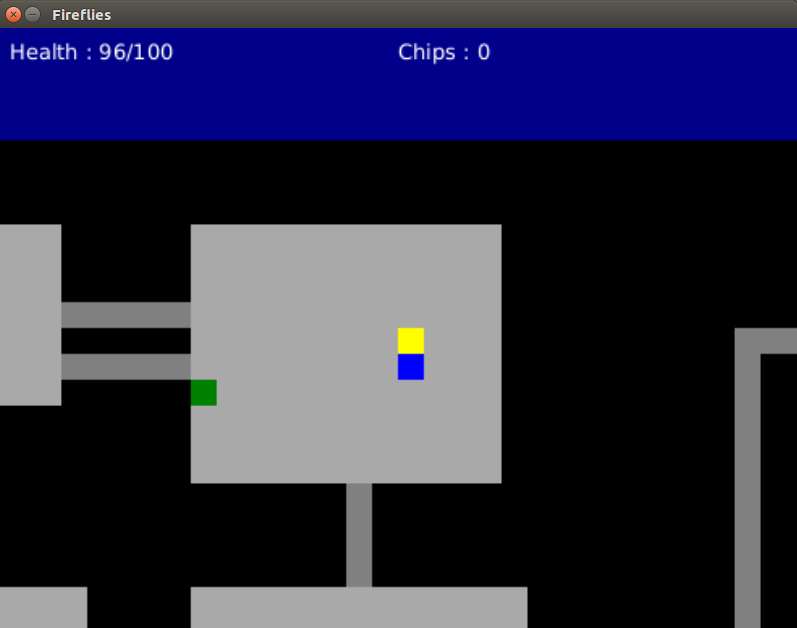
\includegraphics[width=.5\textwidth]{normal-1.png}\hfill
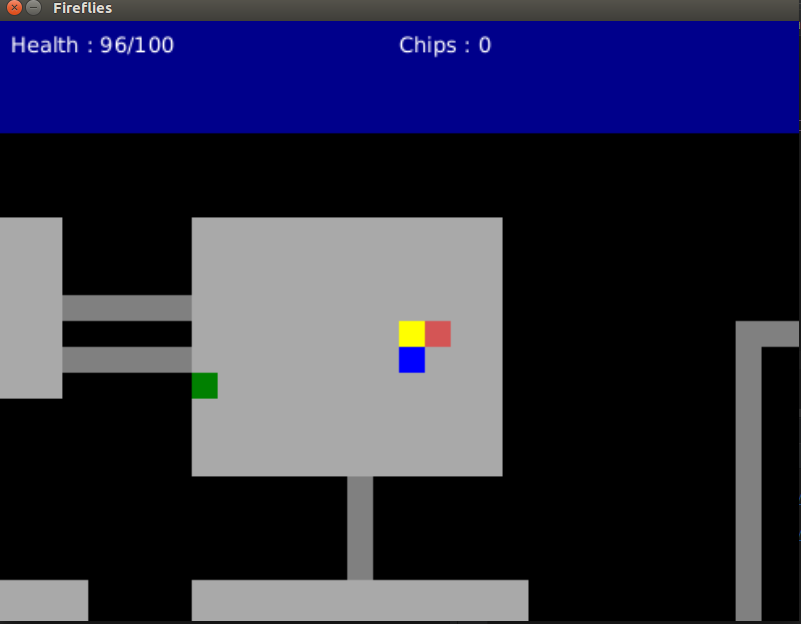
\includegraphics[width=.5\textwidth]{combat-marker.png}\hfill
\vspace*{0.03cm}
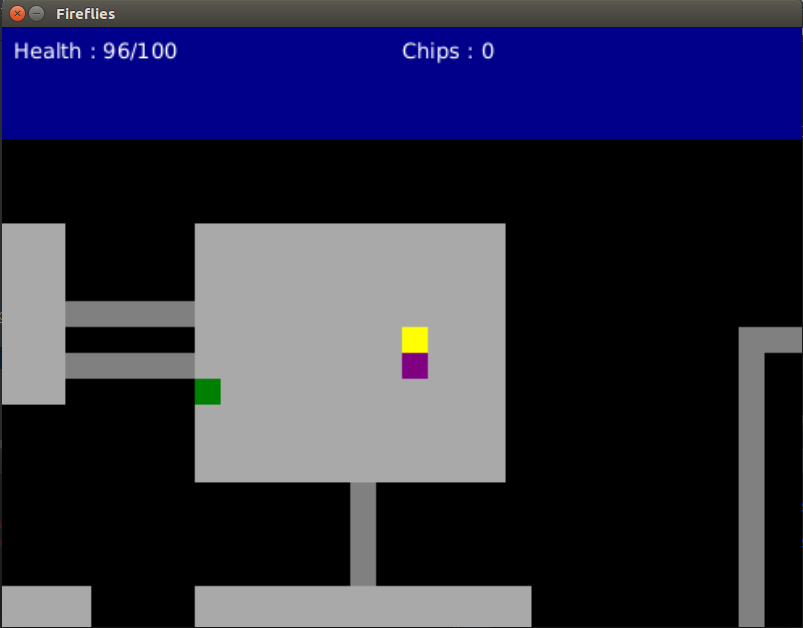
\includegraphics[width=.5\textwidth]{combat-marker-2.png}

\caption{{\em (Upper-left)} Shows the player character {\em (yellow box)} in a normal idle state in a room with enemies; {\em (Upper-right)} Shows the player in the attack state, the red marker shows which side the player's attack is currently pointing; {\em (Center)} Shows the marker currently pointed at the blue enemy.}
\label{fig:combatphase}

\end{figure}

The core combat mechanics in the game is adapted from the mechanics of the traditional {\em rock, paper, and scissors}(RPS) game where 2 players choose from the three (rock, paper, and scissors) per turn and the victor are determined by the very simple rule: rock beats scissors, scissors beats paper, and paper beats rock. We chose to adapt the concept for the combat system of our game because it proves to be one of the most balanced mechanics in a game available, since all the players are given a similar set of tools and rules so that everyone has the same chances of winning given that they know how to play and use their tools correctly. In {\em Fireflies}, the RPS system is implemented in the attacks and defense of both the player and enemy actors, where one attack is stronger than the defense of the other. The rock, paper, and scissors are represented as red, blue, and green element types, respectively. The player may choose to attack using any of the three elements, but the enemies will only have one element for attacking and defense.

The player may be {\em proficient} with an element type(red, blue, green). She may choose to become proficient with only one element at a time. This will increase her damage output to the enemy when attacking with an element that matches her proficiency, but will also increase the damage of an enemy with an element that is stronger the her proficient type. Switching her proficient type requires spending four(4) {\em chips} which can be collected after defeating an enemy. Each enemy drops two(2) chips when their health reaches zero(0).

The game, in its current state, is still open-ended. The player may continue to play in as many levels as she want or until her character's health reaches zero. 

\subsection{Game Controls}
The game Fireflies can be played using keyboard controls. Using the arrow keys will allow the player to move around and explore the map while the space bar will show an indicator and allow the player to attack once an enemy is encountered. 

Once the indicator is shown, the player can choose whether which direction she will attack using the arrow keys. When the player determines which direction she will attack, the player can choose which skill she will use in order to defeat an enemy using the Q, W and E keys. 

The Q key will stand for the “cut” skill which will output a “bleed” effect, the W key being the “stable” which will have a “disarm” effect and the E key will be the “brute” skill which will have a “stun” effect.


\subsection{The Genetic Algorithm}

Every level has a population of enemies, and every enemy in the game has an element that defines their strenth and weaknesses in combat. These elements are, as discussed above, the {\em red}, {\em blue}, and {\em green} elements.

The game's genetic algorithm(GA) resides in the level generator, where the enemies are also generated. The GA takes in the population of enemy {\em non-playable character}(NPC) and evaluates the fitness of every NPC in the population. The NPCs' fitness is based on their remaining {\em health} after the player has exited the level in which they are in. This enables the enemies of the previous level that the player did not or cannot kill or find to get significantly better chances of being a {\em parent} than the other enemy NPCs.

\section{Results}
This chapter presents the results of the project.

\section{Conclusion}
This chapter presents our conclusion to the project, including our recommendations to future researchers.



\bibliographystyle{plain}
\bibliography{biblio}


\end{document}
